\documentclass[12pt, a4paper]{article}\usepackage[]{graphicx}\usepackage[]{color}
% maxwidth is the original width if it is less than linewidth
% otherwise use linewidth (to make sure the graphics do not exceed the margin)
\makeatletter
\def\maxwidth{ %
  \ifdim\Gin@nat@width>\linewidth
    \linewidth
  \else
    \Gin@nat@width
  \fi
}
\makeatother

\definecolor{fgcolor}{rgb}{0.345, 0.345, 0.345}
\newcommand{\hlnum}[1]{\textcolor[rgb]{0.686,0.059,0.569}{#1}}%
\newcommand{\hlstr}[1]{\textcolor[rgb]{0.192,0.494,0.8}{#1}}%
\newcommand{\hlcom}[1]{\textcolor[rgb]{0.678,0.584,0.686}{\textit{#1}}}%
\newcommand{\hlopt}[1]{\textcolor[rgb]{0,0,0}{#1}}%
\newcommand{\hlstd}[1]{\textcolor[rgb]{0.345,0.345,0.345}{#1}}%
\newcommand{\hlkwa}[1]{\textcolor[rgb]{0.161,0.373,0.58}{\textbf{#1}}}%
\newcommand{\hlkwb}[1]{\textcolor[rgb]{0.69,0.353,0.396}{#1}}%
\newcommand{\hlkwc}[1]{\textcolor[rgb]{0.333,0.667,0.333}{#1}}%
\newcommand{\hlkwd}[1]{\textcolor[rgb]{0.737,0.353,0.396}{\textbf{#1}}}%
\let\hlipl\hlkwb

\usepackage{framed}
\makeatletter
\newenvironment{kframe}{%
 \def\at@end@of@kframe{}%
 \ifinner\ifhmode%
  \def\at@end@of@kframe{\end{minipage}}%
  \begin{minipage}{\columnwidth}%
 \fi\fi%
 \def\FrameCommand##1{\hskip\@totalleftmargin \hskip-\fboxsep
 \colorbox{shadecolor}{##1}\hskip-\fboxsep
     % There is no \\@totalrightmargin, so:
     \hskip-\linewidth \hskip-\@totalleftmargin \hskip\columnwidth}%
 \MakeFramed {\advance\hsize-\width
   \@totalleftmargin\z@ \linewidth\hsize
   \@setminipage}}%
 {\par\unskip\endMakeFramed%
 \at@end@of@kframe}
\makeatother

\definecolor{shadecolor}{rgb}{.97, .97, .97}
\definecolor{messagecolor}{rgb}{0, 0, 0}
\definecolor{warningcolor}{rgb}{1, 0, 1}
\definecolor{errorcolor}{rgb}{1, 0, 0}
\newenvironment{knitrout}{}{} % an empty environment to be redefined in TeX

\usepackage{alltt}

%%%%%%%%%%%%%%%%%%%%%%%%%%%%%%%%%%%%%%%%%%%%%%%%%%%%%%%%%%%%%%%%%%%%%%%%%%%%%%%%%%%%%%%%%%%%%%%%
  % dodatkowe pakiety LaTeX'a
\usepackage[OT4]{polski}
\usepackage[utf8]{inputenc}
\usepackage[top=2.5cm, bottom=2.5cm, left=2cm, right=2cm]{geometry}
\usepackage{graphicx}
\usepackage{float}
\usepackage[colorlinks=true, linkcolor=blue]{hyperref}
\usepackage{mathtools}


%%%%%%%%%%%%%%%%%%%%%%%%%%%%%%%%%%%%%%%%%%%%%%%%%%%%%%%%%%%%%%%%%%%%%%%%%%%%%%%%%%%%%%%%%%%%%%%%
% ustawienia globalne


\IfFileExists{upquote.sty}{\usepackage{upquote}}{}
\begin{document}

%%%%%%%%%%%%%%%%%%%%%%%%%%%%%%%%%%%%%%%%%%%%%%%%%%%%%%%%%%%%%%%%%%%%%%%%%%%%%%%%%%%%%%%%%%%%%%%%
  % strona tytulowa
\title{Sprawozdanie 3}
\author{Maciej Łosiewicz \\ album 256319}
\maketitle
\tableofcontents


\section{Zadanie 1}
\subsection{Wskaźniki analizy technicznej}
\subsubsection{Wskaźnik MACD}

\begin{itemize}

\item Jest on członkiem grupy oscylatorów momentum. Wyliczany jest na podstawie kilku średnich kroczących

\item Składa się z dwóch linii - MACD oraz "linii signal"

\item Linia MACD = Śr. długookresowa - śr. krótkookresowa

\item Linia sygnalna = Średnia z linii MACD

\item Jeżeli linia MACD kieruje się w górę to mamy do czynienia z sygnałem pozytywnym, jeśli w dół – z sygnałem negatywnym

\item Linię MACD uznajemy za linię kupna bądź sprzedaży w zależności czy przecina linię sygnalną z dołu czy od góry

\end{itemize}


\subsubsection{Wskaźnik STS/SMI}


\begin{itemize}

\item Jeden ze wskaźników momentum

\item Oblicza stosunek zmiany ceny zamknięcia do różnicy ceny minimalnej i maksymalnej, a wartości te są jeszcze dodatkowo uśredniane za pomocą średniej ruchomej

\item Składa się z dwóch linii – $K$ oraz $D$. 

\item $K$ obliczana jest na podstawie wzoru:

\[
 \%K = 100\dfrac{(C – Min)}{(Max – Min)} 
\]

Gdzie $C$ = cena zamknięcia z bieżącego dnia, $Min$ = cena minimalna z całego okresu, a $Max$ = cena maksymalna z całego okresu

\item $D$ to 3-okresowa średnia krocząca linii $K$, nazywana także szybkim oscylatorem stochastycznym

\end{itemize}


\subsubsection{Wstęga Bollingera}


\begin{itemize}

\item Wskaźnik wstęgi Bollingera wykorzystuje odchylenie standardowe w celu określenia, gdzie może pojawić się możliwy poziom wsparcia lub oporu.

\item Wstęgi Bollingera występują jako dwie linie, zarówno powyżej, jak i poniżej centralnej średniej kroczącej, które obejmują cenę.

\item Wstęgi Bollingera są konstruowane poprzez dodawanie i odejmowanie odchylenia standardowego średniej ruchomej, wskazując zmienność rynku

\end{itemize}



\subsection{Wizualizacja wybranych wskaźników}

Do analizy wybierzmy spółkę Apple

\begin{knitrout}
\definecolor{shadecolor}{rgb}{0.969, 0.969, 0.969}\color{fgcolor}\begin{kframe}
\begin{verbatim}
## [1] "AAPL"
\end{verbatim}
\end{kframe}\begin{figure}[H]

{\centering 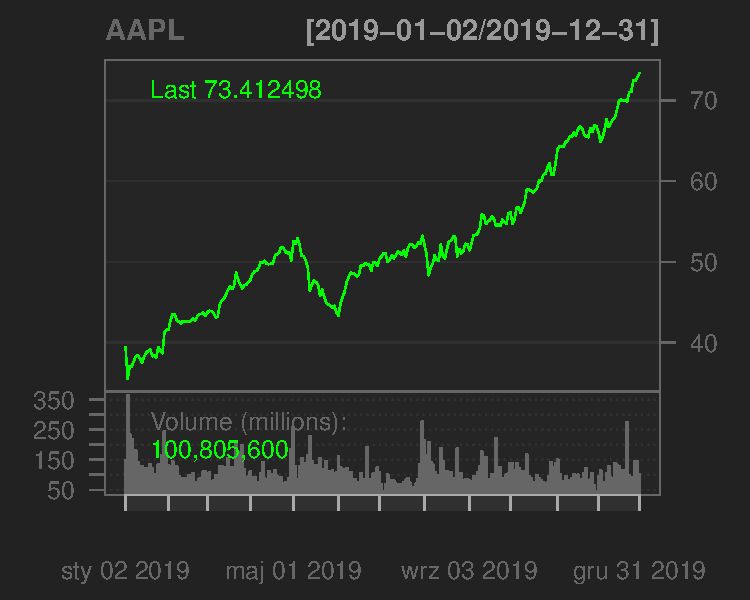
\includegraphics[width=\maxwidth]{figure/unnamed-chunk-1-1} 

}

\caption[Wykres danych AAPL]{Wykres danych AAPL}\label{fig:unnamed-chunk-1}
\end{figure}

\end{knitrout}


\begin{knitrout}
\definecolor{shadecolor}{rgb}{0.969, 0.969, 0.969}\color{fgcolor}\begin{figure}[H]

{\centering 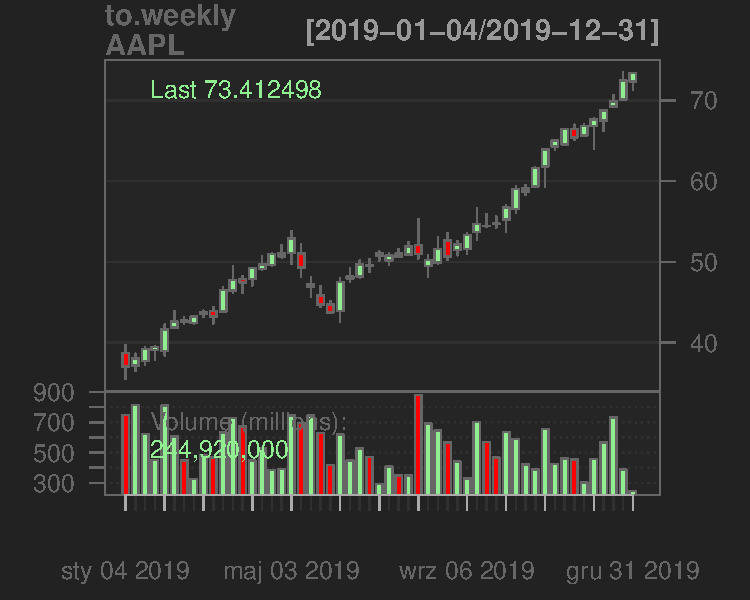
\includegraphics[width=\maxwidth]{figure/unnamed-chunk-2-1} 

}

\caption[Podział danych na zakres tygodniowy]{Podział danych na zakres tygodniowy}\label{fig:unnamed-chunk-2}
\end{figure}

\end{knitrout}

\subsubsection{Wskaźnik MACD}

\begin{knitrout}
\definecolor{shadecolor}{rgb}{0.969, 0.969, 0.969}\color{fgcolor}\begin{figure}[H]

{\centering 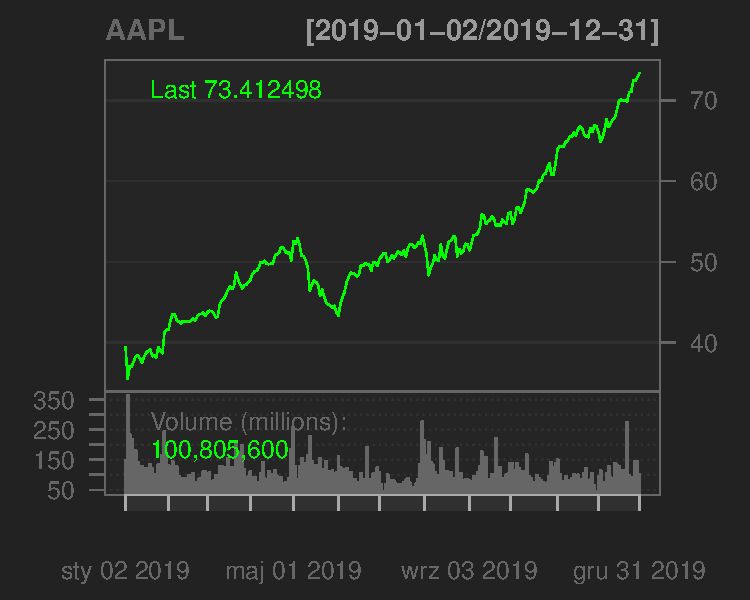
\includegraphics[width=\maxwidth]{figure/unnamed-chunk-3-1} 

}

\caption[Wykres danych ze wskaźnikiem MACD]{Wykres danych ze wskaźnikiem MACD}\label{fig:unnamed-chunk-3-1}
\end{figure}

\begin{figure}[H]

{\centering 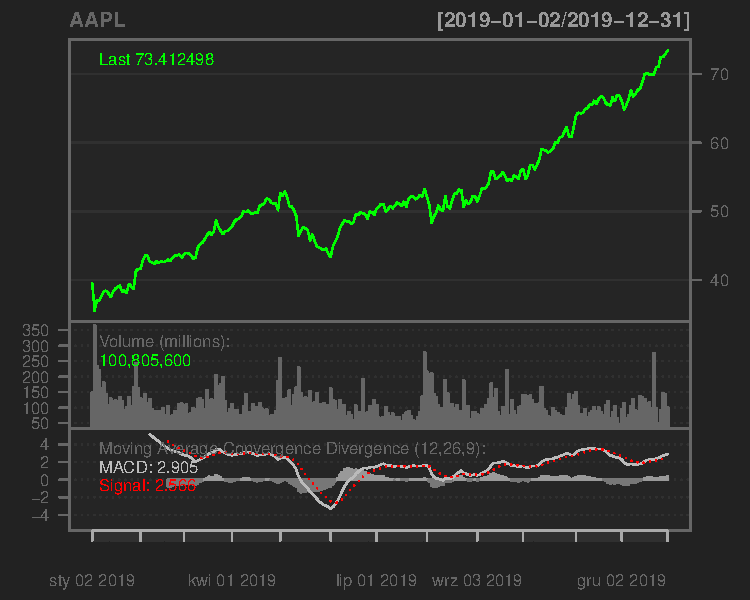
\includegraphics[width=\maxwidth]{figure/unnamed-chunk-3-2} 

}

\caption[Wykres danych ze wskaźnikiem MACD]{Wykres danych ze wskaźnikiem MACD}\label{fig:unnamed-chunk-3-2}
\end{figure}

\end{knitrout}

\begin{itemize}

\item Kiedy linia MACD (czerwona) przecina poziom 0 pokazuje to, że momentum się zmienia i potencjalnie tworzony jest nowy trend. 

\item Gdy dwie linie wskaźnika MACD oddalają się od siebie oznacza to, że rośnie momentum, a gdy są coraz bliżej, to cena traci siłę

\end{itemize}

\subsubsection{Wskaźnik STS/SMI}


\begin{knitrout}
\definecolor{shadecolor}{rgb}{0.969, 0.969, 0.969}\color{fgcolor}\begin{figure}[H]

{\centering 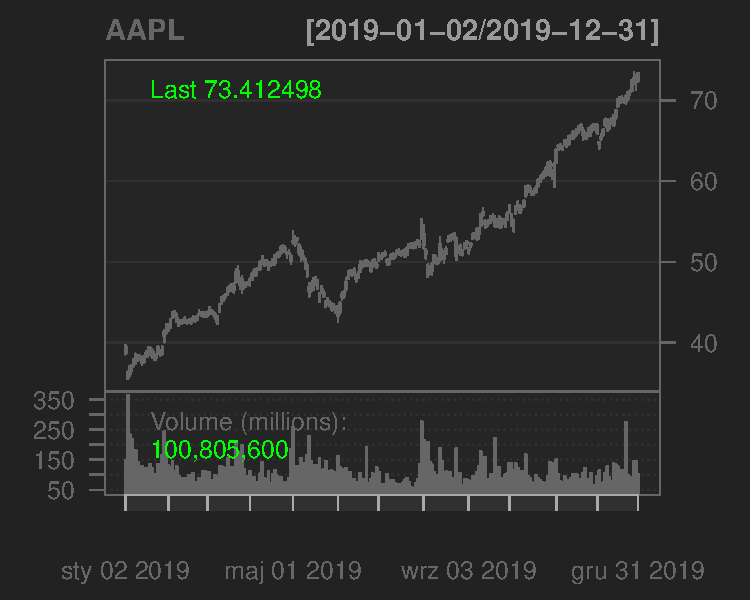
\includegraphics[width=\maxwidth]{figure/unnamed-chunk-4-1} 

}

\caption[Wykres danych ze wskaźnikiem SMI]{Wykres danych ze wskaźnikiem SMI}\label{fig:unnamed-chunk-4-1}
\end{figure}

\begin{figure}[H]

{\centering 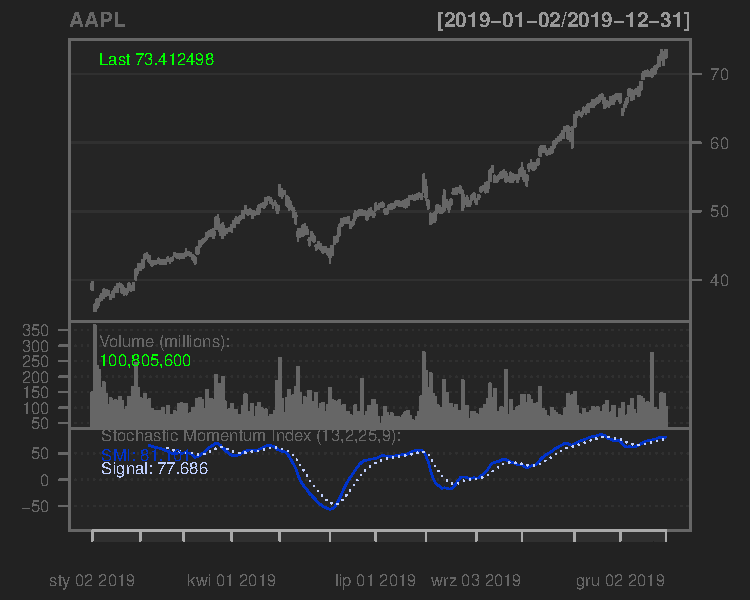
\includegraphics[width=\maxwidth]{figure/unnamed-chunk-4-2} 

}

\caption[Wykres danych ze wskaźnikiem SMI]{Wykres danych ze wskaźnikiem SMI}\label{fig:unnamed-chunk-4-2}
\end{figure}

\begin{figure}[H]

{\centering 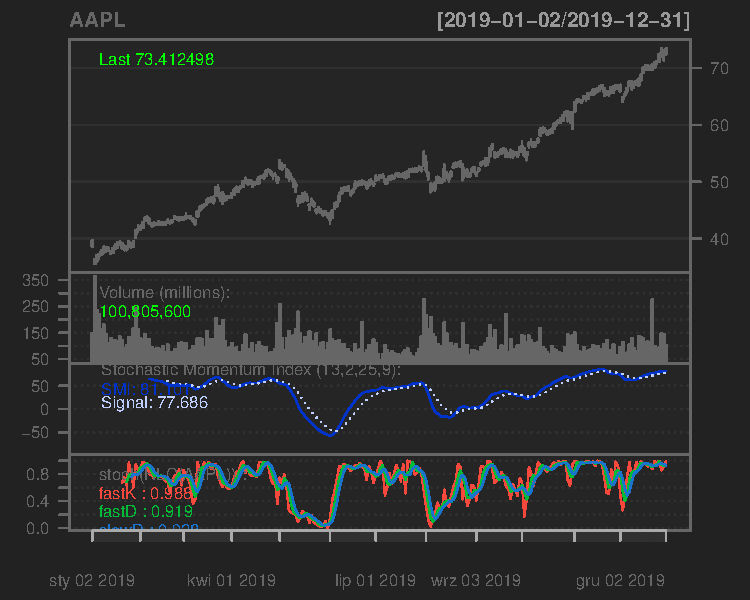
\includegraphics[width=\maxwidth]{figure/unnamed-chunk-4-3} 

}

\caption[Wykres danych ze wskaźnikiem SMI]{Wykres danych ze wskaźnikiem SMI}\label{fig:unnamed-chunk-4-3}
\end{figure}

\end{knitrout}


\begin{itemize}

\item Ten oscylator stochastyczny zbudowany jest z dwóch linii - oscylatora wolnego $K$ (niebieska linia) oraz szybkiego $D$

\item Kiedy linia $D$ przecina $K$ od dołu, należy kupować akcję, i analogicznie gdy przecina od góry należy myśleć o sprzedaży

\end{itemize}

\subsubsection{Wstęga Bollingera}

\begin{knitrout}
\definecolor{shadecolor}{rgb}{0.969, 0.969, 0.969}\color{fgcolor}\begin{figure}[H]

{\centering 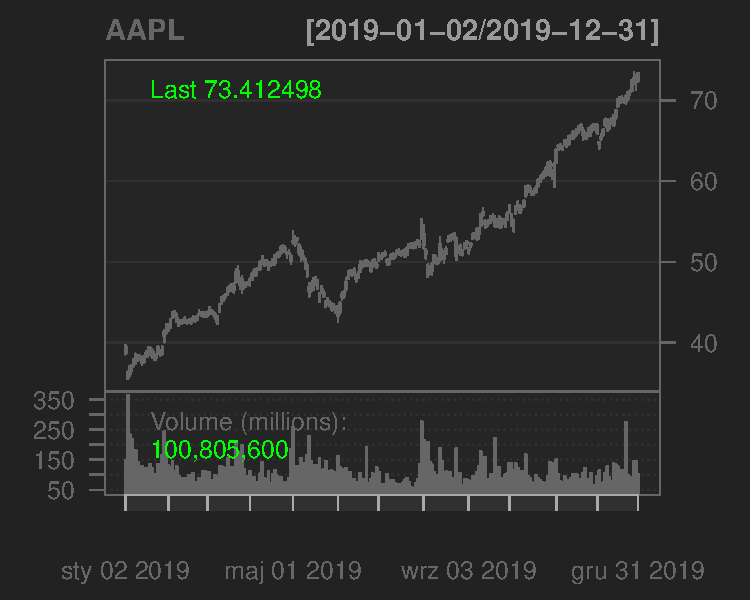
\includegraphics[width=\maxwidth]{figure/unnamed-chunk-5-1} 

}

\caption[Wykres danych ze wstęgą Bollingera]{Wykres danych ze wstęgą Bollingera}\label{fig:unnamed-chunk-5-1}
\end{figure}

\begin{figure}[H]

{\centering 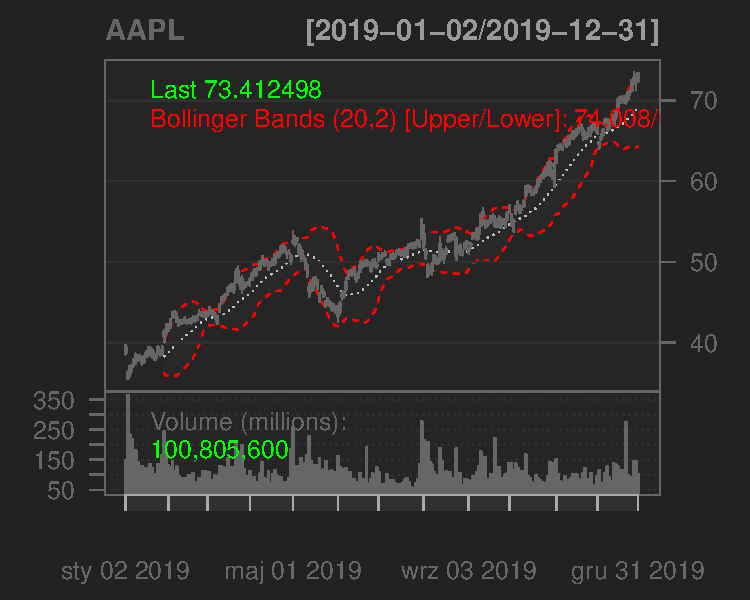
\includegraphics[width=\maxwidth]{figure/unnamed-chunk-5-2} 

}

\caption[Wykres danych ze wstęgą Bollingera]{Wykres danych ze wstęgą Bollingera}\label{fig:unnamed-chunk-5-2}
\end{figure}

\end{knitrout}


\begin{itemize}

\item Szerokość wstęgi zależy od odchylenia standardowego. Przy zwężeniu należy spodziewać się zmiany cen, a po tym rozszerzenie i stabliność notowań.

\end{itemize}

\subsection{Wybór parametrów}

\subsubsection{Wskaźnik MACD}

\begin{knitrout}
\definecolor{shadecolor}{rgb}{0.969, 0.969, 0.969}\color{fgcolor}\begin{figure}[H]

{\centering 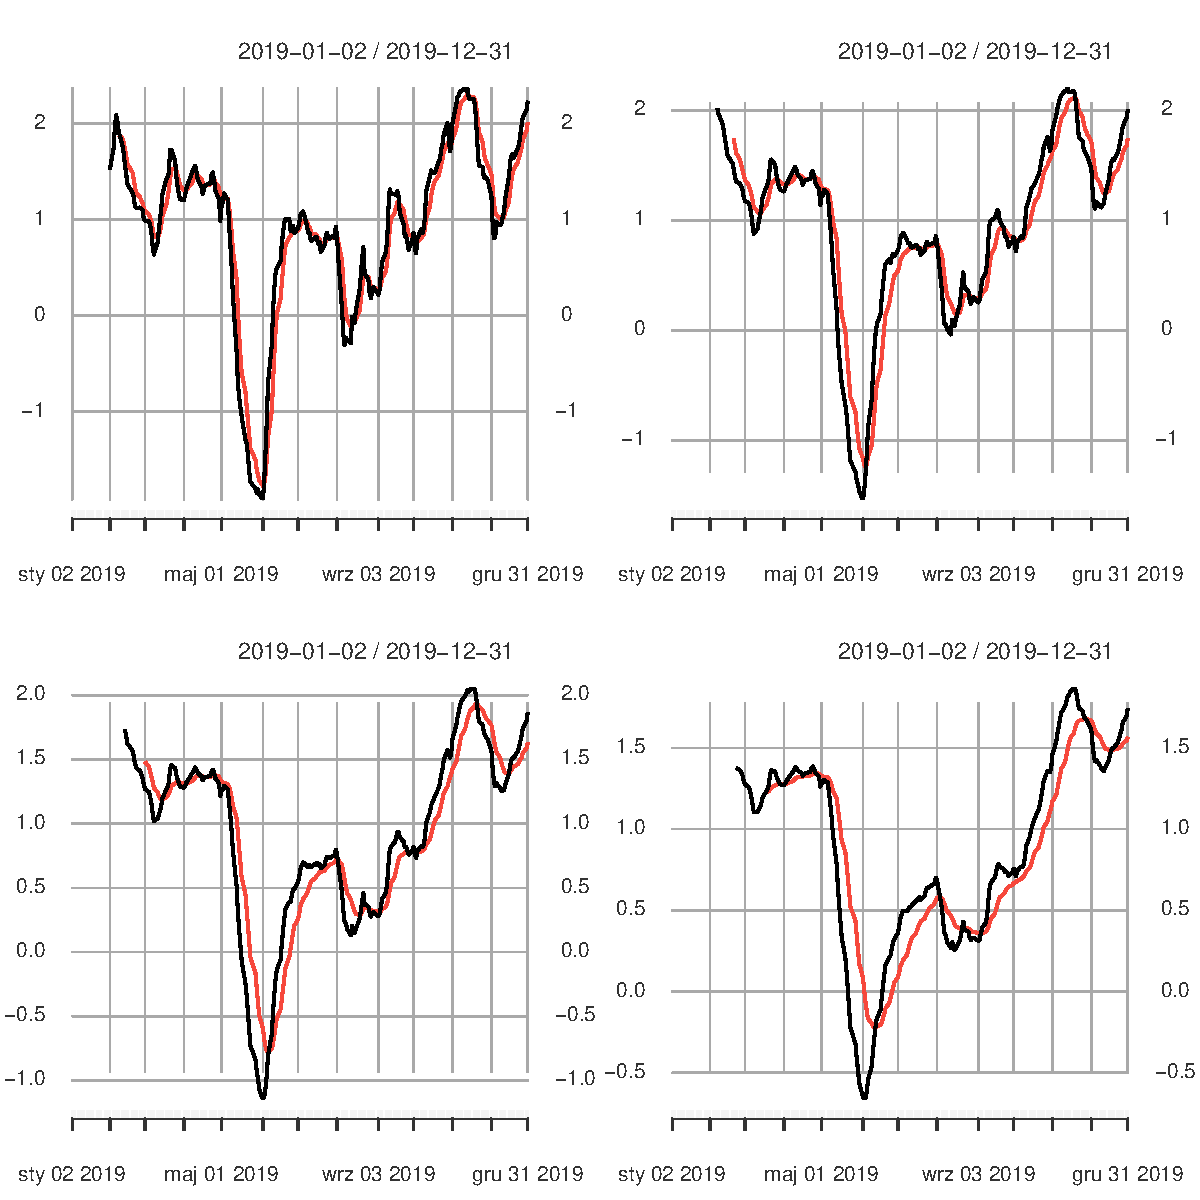
\includegraphics[width=\maxwidth]{figure/unnamed-chunk-6-1} 

}

\caption[Wykres MACD dla różnych parametrów]{Wykres MACD dla różnych parametrów}\label{fig:unnamed-chunk-6}
\end{figure}

\end{knitrout}

Przy zwiększeniu wartości parametrów widzimy oddalenie się linii co symbolizuje wzrost momentum, a co za tym idzie trend zyskuje siłę. Analogicznie dla małych parametrów lniie są blisko siebie co symbolizuje że cena traci siłę.

\subsubsection{Wskaźnik SMI}

\begin{knitrout}
\definecolor{shadecolor}{rgb}{0.969, 0.969, 0.969}\color{fgcolor}\begin{figure}[H]

{\centering 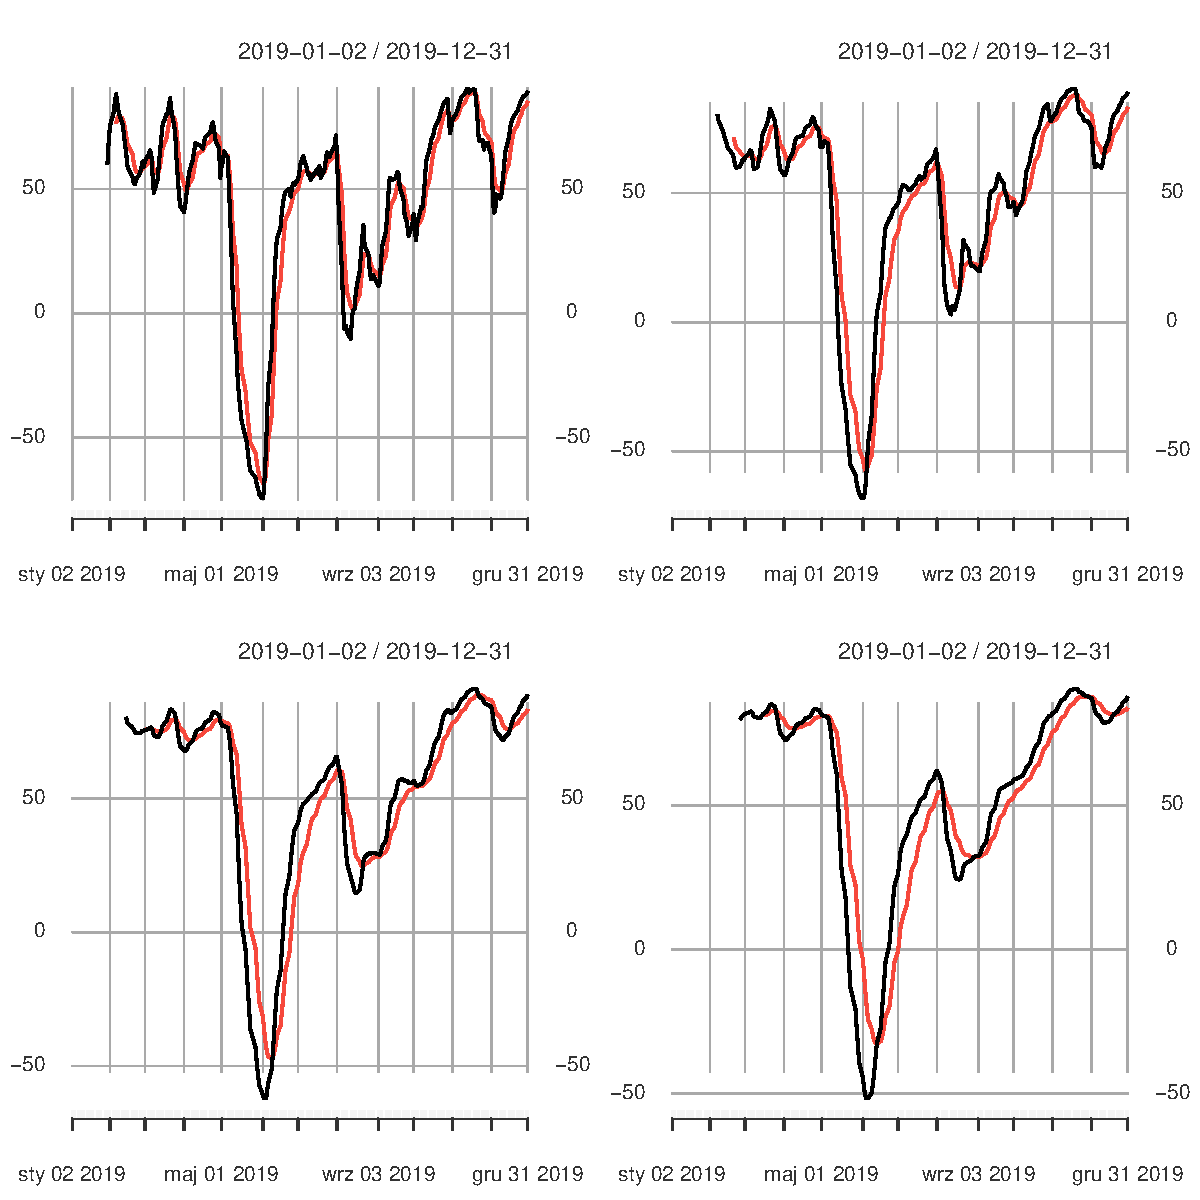
\includegraphics[width=\maxwidth]{figure/unnamed-chunk-7-1} 

}

\caption[Wykres SMI dla różnych parametrów]{Wykres SMI dla różnych parametrów}\label{fig:unnamed-chunk-7}
\end{figure}

\end{knitrout}

Tak jak można się było domyślić, zwiększenie parametrów też i w tym wypadku oddala od siebie linie $K$ i $D$


\subsubsection{Wstęga Bollingera}

\begin{knitrout}
\definecolor{shadecolor}{rgb}{0.969, 0.969, 0.969}\color{fgcolor}\begin{figure}[H]

{\centering 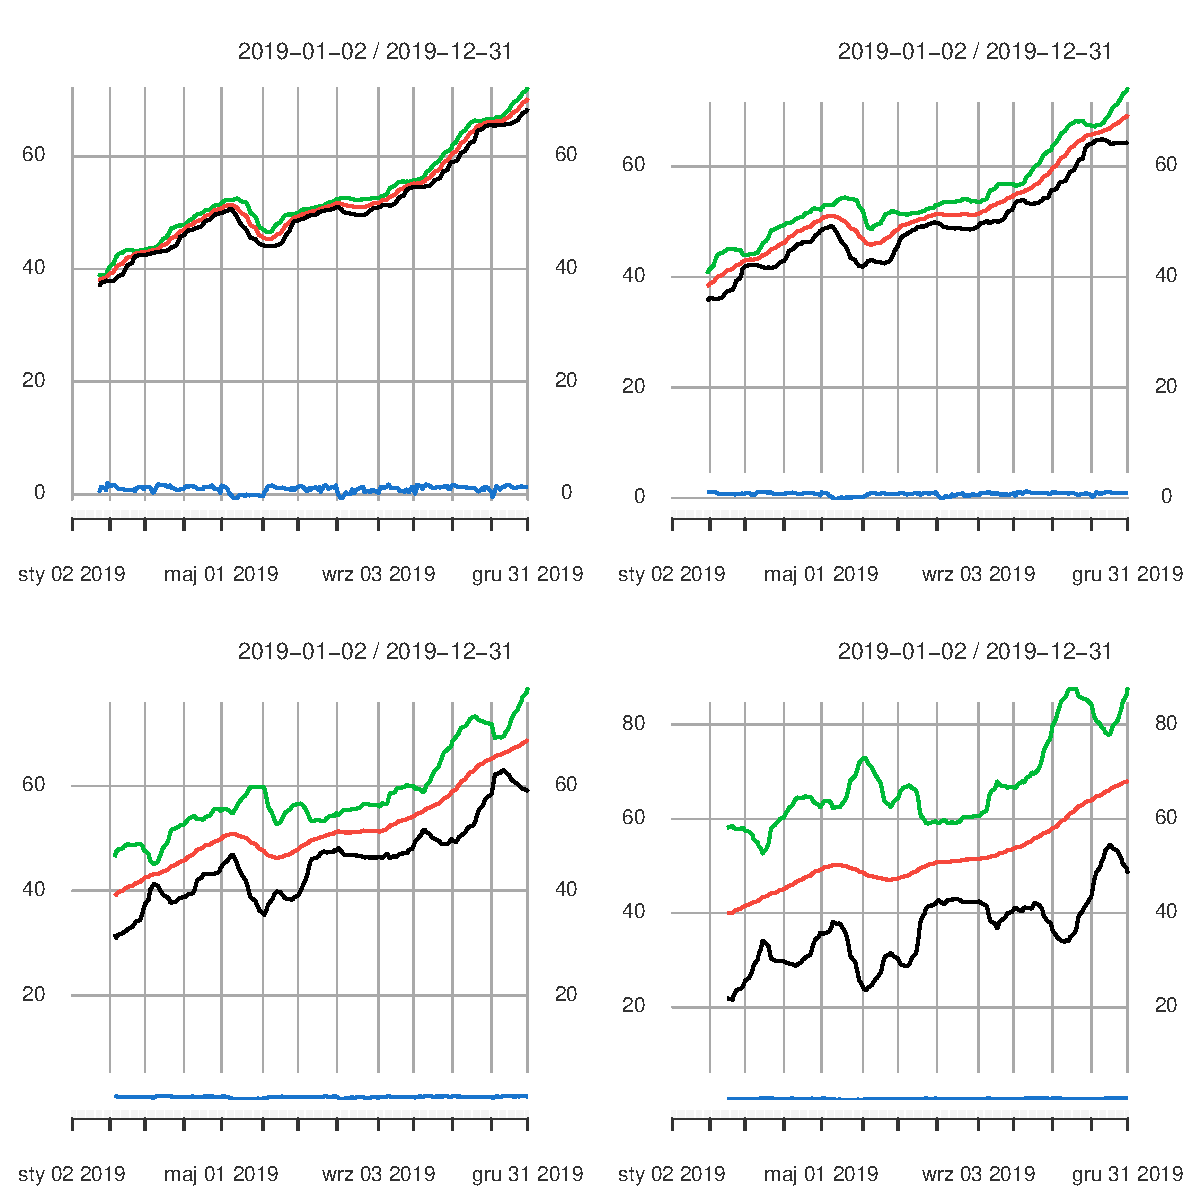
\includegraphics[width=\maxwidth]{figure/unnamed-chunk-8-1} 

}

\caption[Wykres wstęgi dla różnych parametrów]{Wykres wstęgi dla różnych parametrów}\label{fig:unnamed-chunk-8}
\end{figure}

\end{knitrout}

Tak jak w poprzednich przypadkach, zwiększenie parametrów drastycznie zwiększa szerokość wstęgi.

\section{Zadanie 2}

\subsection{Weryfikacja stacjonarności danych}

\begin{knitrout}
\definecolor{shadecolor}{rgb}{0.969, 0.969, 0.969}\color{fgcolor}\begin{figure}[H]

{\centering 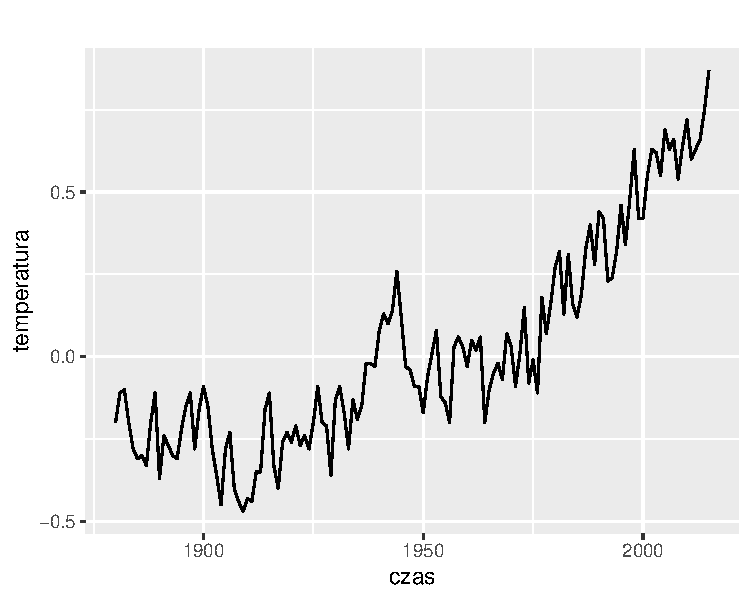
\includegraphics[width=\maxwidth]{figure/unnamed-chunk-9-1} 

}

\caption[Wykres danych]{Wykres danych}\label{fig:unnamed-chunk-9-1}
\end{figure}

\begin{figure}[H]

{\centering 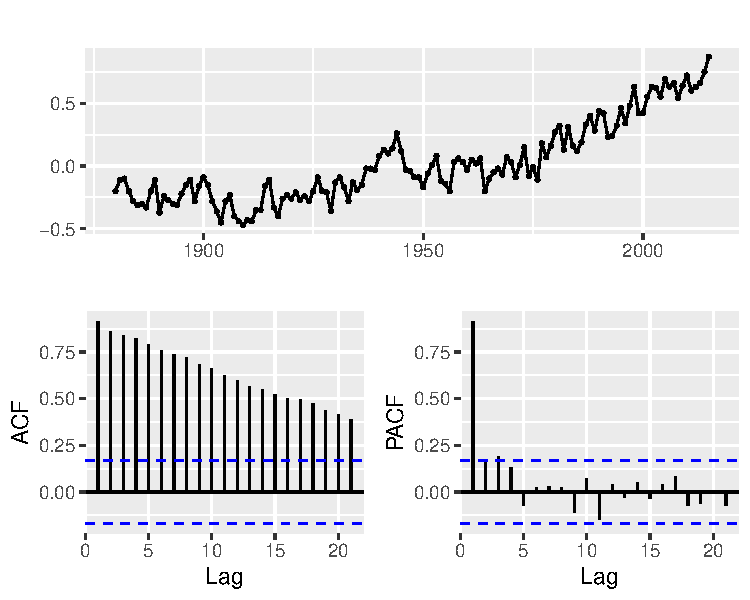
\includegraphics[width=\maxwidth]{figure/unnamed-chunk-9-2} 

}

\caption[Wykres danych]{Wykres danych}\label{fig:unnamed-chunk-9-2}
\end{figure}

\end{knitrout}

Łatwo zauważyć że ACF maleje, a więc korelacja także maleje, i to w sposób podobny do liniowego. Natomiast dla PACF widać że pierwsza obserwacja wynosi prawie 1, co oznacza, że cząstkowa autokorelacja wskazuje nam istnienie trendu

Przejdźmy do wielomianowej transformacji danych

\begin{knitrout}
\definecolor{shadecolor}{rgb}{0.969, 0.969, 0.969}\color{fgcolor}

{\centering 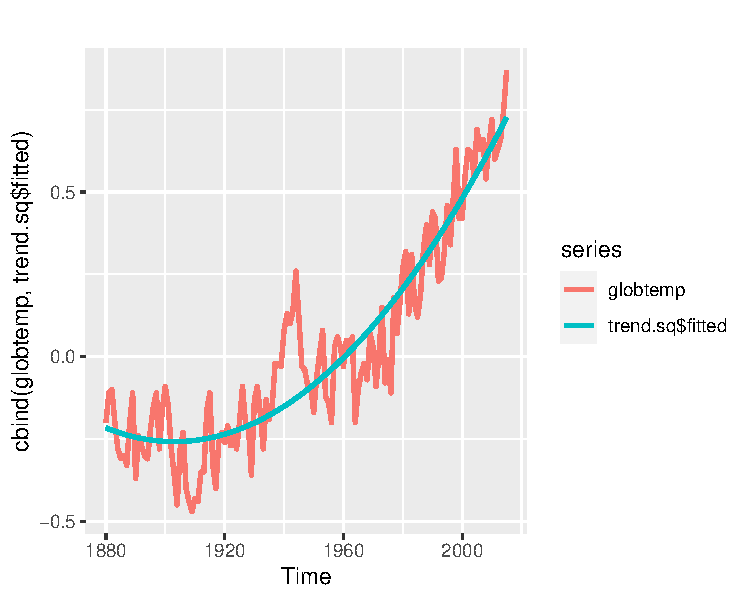
\includegraphics[width=\maxwidth]{figure/unnamed-chunk-10-1} 

}




{\centering 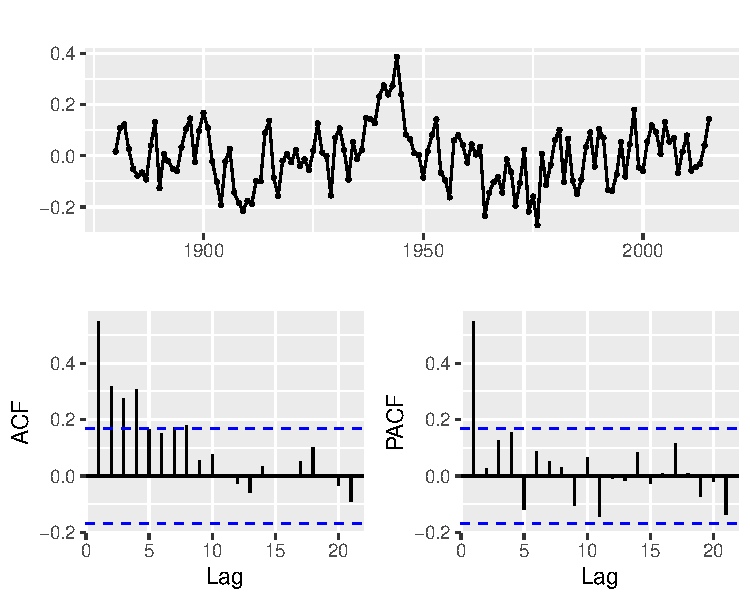
\includegraphics[width=\maxwidth]{figure/unnamed-chunk-10-2} 

}


\end{knitrout}

Z wykresów ACF i PACF identyfikujemy MA(4) oraz AR(1)

\subsection{Estymacja modelu}

Wykorzystamy metody Yule'a-Walkera oraz metodę największej wiarygodności.

Najpierw dla Yule'a-Walkera:

\begin{knitrout}
\definecolor{shadecolor}{rgb}{0.969, 0.969, 0.969}\color{fgcolor}\begin{kframe}
\begin{verbatim}
## 
## Call:
## ar(x = globtemp.r, aic = FALSE, order.max = 1, method = "yw")
## 
## Coefficients:
##      1  
## 0.5479  
## 
## Order selected 1  sigma^2 estimated as  0.00926
##             [,1]
## [1,] 0.005222103
\end{verbatim}
\end{kframe}
\end{knitrout}

Następnie dla mle:

\begin{knitrout}
\definecolor{shadecolor}{rgb}{0.969, 0.969, 0.969}\color{fgcolor}\begin{kframe}
\begin{verbatim}
## 
## Call:
## ar(x = globtemp.r, aic = FALSE, order.max = 1, method = "mle")
## 
## Coefficients:
##      1  
## 0.5504  
## 
## Order selected 1  sigma^2 estimated as  0.009077
##             [,1]
## [1,] 0.005119081
\end{verbatim}
\end{kframe}
\end{knitrout}

Teraz sprawdźmy różnicę między tymi dwoma metodami:

\begin{knitrout}
\definecolor{shadecolor}{rgb}{0.969, 0.969, 0.969}\color{fgcolor}\begin{kframe}
\begin{verbatim}
##              [,1]
## [1,] 0.0001030225
\end{verbatim}
\end{kframe}
\end{knitrout}

\subsection{Przedziały ufności}

Teraz skonstruujemy przedziały ufności dla modelu AR(4) %(dla AR(1) w modelu wielomianowym pojawia się błąd)


\begin{knitrout}
\definecolor{shadecolor}{rgb}{0.969, 0.969, 0.969}\color{fgcolor}\begin{kframe}
\begin{verbatim}
## 
## 	One-sample asymptotic mean test
## 
## data:  yw$ar
## statistic = -2.1602, p-value = 0.03076
## alternative hypothesis: true mean is not equal to 0
## 95 percent confidence interval:
##  -0.38015707 -0.01847217
## sample estimates:
##       mean 
## -0.1993146
## 
## 	One-sample asymptotic mean test
## 
## data:  mle$ar
## statistic = -2.259, p-value = 0.02389
## alternative hypothesis: true mean is not equal to 0
## 95 percent confidence interval:
##  -0.39123015 -0.02772722
## sample estimates:
##       mean 
## -0.2094787
\end{verbatim}
\end{kframe}
\end{knitrout}

\subsection{Weryfikacja poprawności dopasowania}

\begin{knitrout}
\definecolor{shadecolor}{rgb}{0.969, 0.969, 0.969}\color{fgcolor}\begin{kframe}
\begin{verbatim}
## 
## 	Box-Pierce test
## 
## data:  res.yw
## X-squared = 0.038685, df = 1, p-value = 0.8441
## 
## 	Box-Pierce test
## 
## data:  res.yw
## X-squared = 14.665, df = 16, p-value = 0.5493
## 
## 	Box-Pierce test
## 
## data:  res.mle
## X-squared = 0.010451, df = 1, p-value = 0.9186
## 
## 	Box-Pierce test
## 
## data:  res.mle
## X-squared = 14.855, df = 16, p-value = 0.5353
## 
## 	Box-Ljung test
## 
## data:  res.yw
## X-squared = 0.039578, df = 1, p-value = 0.8423
## 
## 	Box-Ljung test
## 
## data:  res.yw
## X-squared = 16.453, df = 16, p-value = 0.4218
## 
## 	Box-Ljung test
## 
## data:  res.mle
## X-squared = 0.010692, df = 1, p-value = 0.9176
## 
## 	Box-Ljung test
## 
## data:  res.mle
## X-squared = 16.675, df = 16, p-value = 0.4069
\end{verbatim}
\end{kframe}
\end{knitrout}

Jak widać z testów mamy tylko po jednej kolumnie która znajduje się poza naszym zasięgiem.

\subsection{Prognoza}

Wykonajmy prognozę dla kolejnych wykresów:

\begin{knitrout}
\definecolor{shadecolor}{rgb}{0.969, 0.969, 0.969}\color{fgcolor}

{\centering 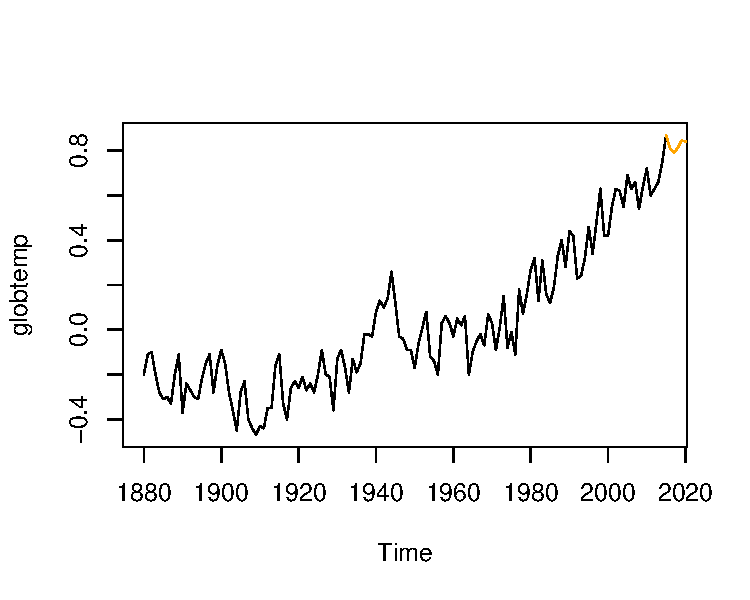
\includegraphics[width=\maxwidth]{figure/unnamed-chunk-16-1} 

}




{\centering 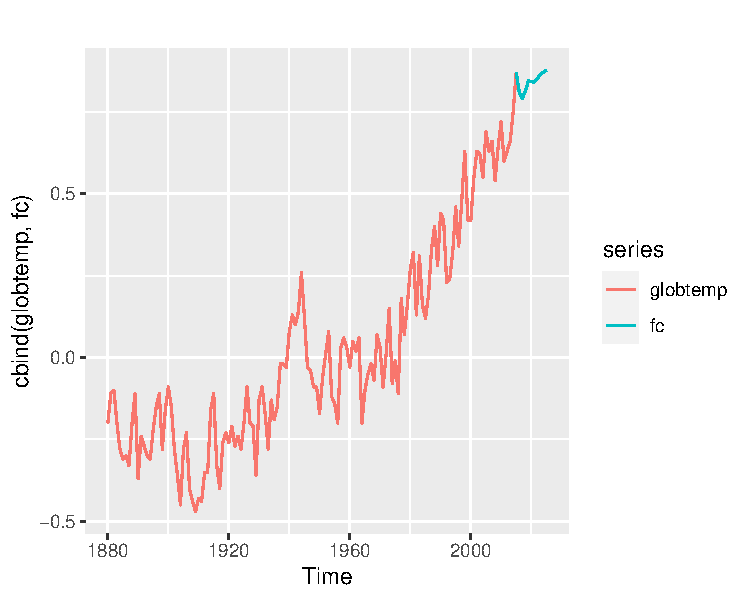
\includegraphics[width=\maxwidth]{figure/unnamed-chunk-16-2} 

}




{\centering 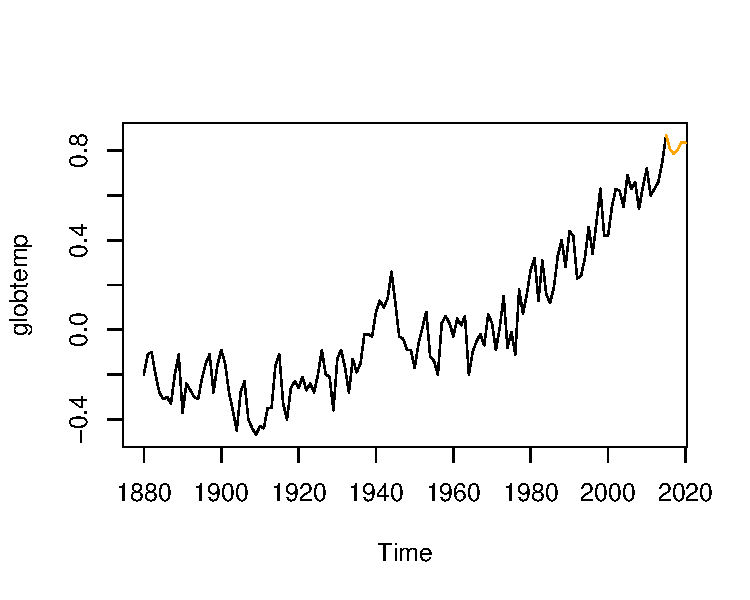
\includegraphics[width=\maxwidth]{figure/unnamed-chunk-16-3} 

}




{\centering 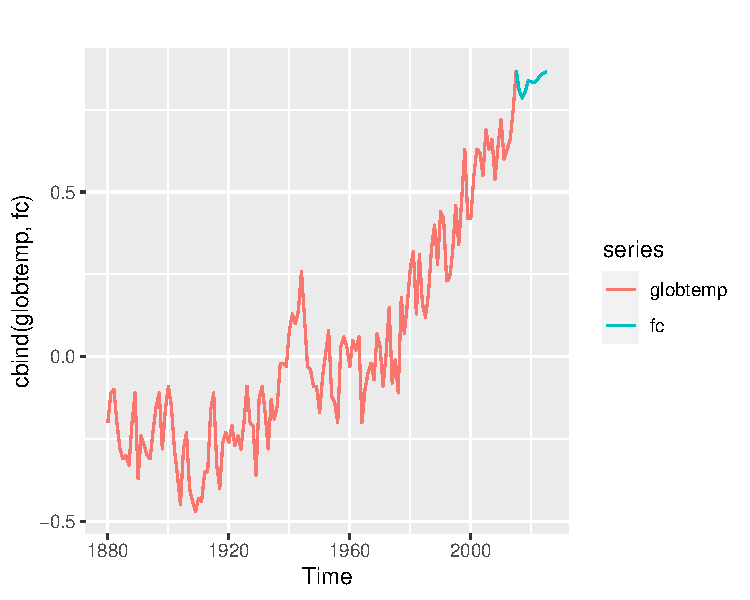
\includegraphics[width=\maxwidth]{figure/unnamed-chunk-16-4} 

}


\end{knitrout}



\end{document}

